\documentclass[conference]{IEEEtran}
\IEEEoverridecommandlockouts

\usepackage[utf8]{inputenc}
\usepackage[T1]{fontenc}
\usepackage{cite}
\usepackage{amsmath,amssymb}
\usepackage{graphicx}
\usepackage{xcolor}
\usepackage{array}
\usepackage{tabularx}
\usepackage{ragged2e}
\usepackage{url}
\usepackage[hidelinks]{hyperref}
\usepackage{tikz}
\usetikzlibrary{positioning, arrows.meta, calc, fit}

\newcolumntype{Y}{>{\RaggedRight\arraybackslash}X}
\newcolumntype{P}[1]{>{\RaggedRight\arraybackslash}p{#1}}
% Starts a new, centered row of author blocks (IEEEtran has no built-in command for this).
\makeatletter
\newcommand{\linebreakand}{\end{@IEEEauthorhalign}\hfill\mbox{}\par\mbox{}\hfill\begin{@IEEEauthorhalign}}
\makeatother

\begin{document}

\title{AI Methods for Health Insurance Claim Denial Analysis and Appeal Support: A Review and a Policy-Grounded Framework}

\author{
\IEEEauthorblockN{Pragallapati Saketh}
\IEEEauthorblockA{\textit{Dept. of Computer Science and Engineering}\\
\textit{Chaitanya Bharathi Institute of Technology}\\
Hyderabad, India\\
pragallapati.saketh@gmail.com}
\and
\IEEEauthorblockN{Saketh Vemulapati}
\IEEEauthorblockA{\textit{Dept. of Computer Science and Engineering}\\
\textit{Chaitanya Bharathi Institute of Technology}\\
Hyderabad, India\\
sakethvemulapati3233@gmail.com}
\linebreakand
\IEEEauthorblockN{A. Sangeetha}
\IEEEauthorblockA{\textit{Assistant Professor, Dept. of CSE}\\
\textit{Chaitanya Bharathi Institute of Technology}\\
Hyderabad, India\\
asangeetha\_cse@cbit.ac.in}
}

\maketitle

\begin{abstract}
A policyholder whose health insurance claim is denied has to find out which policy provisions the insurer relied on, check whether the medical and billing records support the stated reason, and see whether an exception or a regulatory protection applies. Several lines of artificial intelligence (AI) research cover parts of this work. They extract rules from policy text, link clinical terms to standard codes, retrieve evidence from health records, predict appeal outcomes, reason over policy conditions, and draft appeal letters. We review twenty-five works on AI for insurance claims and appeals and on the retrieval, argumentation, and evaluation methods they rely on, and we compare the claims studies by task, modeling approach, knowledge source, evidence traceability, evaluation design, and human oversight. Each study handles one stage of the problem. Models often reach correct final decisions with weak justifications, and generated appeal letters often contain unsupported statements or fabricated references. None of the studies links the denial notice, the governing policy clauses, the case evidence, and the appeal draft in one traceable process. Based on these findings, we propose a policy-grounded workflow for Indian retail health insurance. It sends each denial to an investigation specific to its category, records the evidence for and against each finding, and leaves the final decision to a qualified reviewer. We also describe the knowledge resources built from Indian policy wordings and public code sets, and a set of component-level benchmarks with defined metrics.
\end{abstract}

\begin{IEEEkeywords}
Appeal support, argumentation, claim denial analysis, explainable artificial intelligence, health insurance, large language models, multi-agent systems, retrieval-augmented generation
\end{IEEEkeywords}

\section{Introduction}
\label{sec:intro}
A health insurance policy describes its coverage through definitions, benefits, conditions, exclusions, limits, and waiting periods, and many exclusions carry exceptions of their own. When an insurer denies a claim (in Indian practice, \emph{repudiates} it), the policyholder needs answers to a few practical questions. What reason did the insurer give, and which clauses of which policy version does it rest on? Do the medical records establish the facts that matter? Could an exception or a regulatory protection change the outcome? The answers are scattered across the policy wording, the denial letter, discharge summaries, diagnostic reports, itemized bills, the proposal form, and correspondence. These documents use different formats and terms, and they record facts at different levels of detail.

AI research has addressed parts of this problem separately. Machine-learning models rank denied claims by how likely they are to be overturned. Information extraction picks out denial reasons and clinical entities. Retrieval-augmented generation (RAG), where a language model answers from passages retrieved from a document collection~\cite{lewis2020}, can find the relevant policy text. Multi-agent systems split a large assessment into smaller tasks, each handled by a separate large language model (LLM) component, and symbolic or argumentation-based methods state conditions and exceptions explicitly. LLMs can also write draft appeal letters from verified findings.

These capabilities solve different problems. A model that predicts appeal success cannot say which policy rule was misapplied. A retrieved clause may come from an older policy version, or it may leave out an exception printed elsewhere in the document. A well-written appeal letter can still contain facts nobody checked or references that do not exist. Whether a system gives reliable appeal support depends on how its parts are joined and how each part is tested.

We examine the literature with these issues in mind, because the review informs the design of an appeal-support system for Indian retail health insurance. The paper makes four contributions:
\begin{itemize}
    \item a task-oriented taxonomy of AI methods relevant to analyzing denied health insurance claims (Section~\ref{sec:context});
    \item a review and structured comparison of fourteen studies on policy knowledge extraction, retrieval, medical entity linkage, clinical evidence assessment, denial triage, logic-based reasoning, and appeal generation (Sections~\ref{sec:review} and~\ref{sec:comparison});
    \item a set of open research problems, each paired with a research direction (Section~\ref{sec:gaps});
    \item a policy-grounded workflow for Indian retail health insurance, with its knowledge resources, benchmarks, and evaluation metrics (Section~\ref{sec:framework}).
\end{itemize}

Section~\ref{sec:method} defines the scope of the review, and Section~\ref{sec:context} describes the denial-analysis task. Section~\ref{sec:review} reviews the studies in the order in which a denial workflow would use them. Section~\ref{sec:comparison} compares them, and Section~\ref{sec:gaps} sets out the open problems. Section~\ref{sec:framework} presents the proposed framework, Section~\ref{sec:limitations} discusses its limitations, and Section~\ref{sec:conclusion} concludes.

\section{Scope of the Review}
\label{sec:method}
We selected studies that apply AI to health insurance claims processing, coverage assessment, or denial appeals. Each falls into at least one of these areas: policy knowledge extraction, medical entity linkage, clinical evidence retrieval, multi-agent medical-necessity assessment, machine-learning denial triage, LLM-based appeal drafting, RAG-based insurance assistance, and logic-based claim adjudication. The areas match the stages of the workflow proposed in Section~\ref{sec:framework}. Fourteen studies make up the core of the review, and they are the studies reviewed in Section~\ref{sec:review} and compared in Section~\ref{sec:comparison}.

The review also draws on eleven methodological works that are not themselves about insurance. They cover retrieval-augmented generation, BM25 ranking, reciprocal rank fusion, and the BERTScore metric; argumentation theory, through Toulmin's model of argument and a review of legal reasoning as argumentation; hallucination in text generation; the evaluation of citations in generated text, of retrieval-augmented systems, and of LLM output through G-Eval; and human reliance on automated recommendations. We use these works to explain the concepts and metrics on which the analysis and the proposed framework depend, and we do not include them in the comparison.

We examine each core study along six dimensions: the target task; its input data and knowledge sources; the modeling approach; how evidence is represented and traced back to its source; the evaluation design; and its limitations for supporting appeals after a denial. The studies use different datasets, tasks, and evaluation protocols, so we report their results individually and do not pool them. Throughout, the starting point is a claim that has already been denied. Work on claims processing before payment, such as predicting which claims will need rework~\cite{kumar2010}, is discussed only where its methods carry over.

\section{The Denial-Analysis Task}
\label{sec:context}
Analyzing a denial means answering a chain of dependent questions. First, the stated reason has to be identified and matched to the policy clauses it refers to. Next come the case facts, established from the records, with a note of anything missing or contradictory. The analysis then decides whether those facts meet a coverage condition, trigger an exclusion, or establish an exception. Only when a challenge is supportable are the evidence and the policy language put together into an appeal.

Denial reasons recur in a small number of types. Following the denial-reason taxonomy built for the proposed framework (Section~\ref{sec:framework}), we use seven categories: (1)~medical necessity; (2)~pre-existing disease (PED) and waiting periods; (3)~policy exclusions; (4)~financial limits such as room-rent caps, sub-limits, and non-payable items; (5)~missing documentation; (6)~administrative or procedural grounds such as late intimation; and (7)~eligibility and continuity of coverage. The categories need different evidence. A medical-necessity denial turns on clinical records and guidelines, while a waiting-period denial turns mostly on dates.

Across these categories, the literature relies on five capabilities:
\begin{enumerate}
    \item \textit{Document understanding}, which extracts facts from policies, denial letters, clinical records, and administrative documents.
    \item \textit{Knowledge retrieval}, which finds the relevant policy clauses, definitions, guidelines, and evidence passages.
    \item \textit{Evidence assessment}, which separates information that supports a finding from information that contradicts it, is missing, or is uncertain.
    \item \textit{Policy-grounded reasoning}, which checks conditions, exclusions, exceptions, dates, and amounts against the policy terms.
    \item \textit{Appeal drafting and oversight}, which prepares a draft whose statements each point to a source.
\end{enumerate}

Fig.~\ref{fig:taxonomy} groups the reviewed research into four areas that correspond to these capabilities, along with the problems the areas share. It classifies research; it does not describe a system.

\begin{figure*}[!t]
\centering
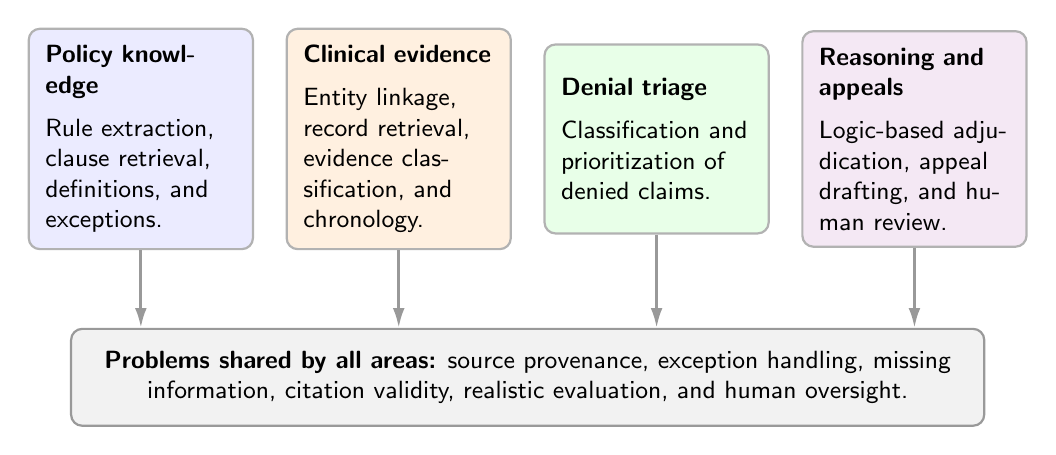
\begin{tikzpicture}[
  node distance=0.4cm,
  card/.style={draw=black!30, thick, rounded corners=4pt, align=left,
    text width=0.2\textwidth, minimum height=2.4cm, inner sep=6pt, font=\small\sffamily},
  challenge/.style={draw=black!40, thick, rounded corners=4pt, align=flush center,
    text width=0.91\textwidth, minimum height=1cm, inner sep=8pt, font=\small\sffamily},
  link/.style={-{Latex[length=2.5mm, width=1.5mm]}, draw=gray!80, line width=1pt}
]
\node[card, fill=blue!8] (a) {\textbf{Policy knowledge}\\[0.5em] Rule extraction, clause retrieval, definitions, and exceptions.};
\node[card, fill=orange!12, right=of a] (b) {\textbf{Clinical evidence}\\[0.5em] Entity linkage, record retrieval, evidence classification, and chronology.};
\node[card, fill=green!9, right=of b] (c) {\textbf{Denial triage}\\[0.5em] Classification and prioritization of denied claims.};
\node[card, fill=violet!9, right=of c] (d) {\textbf{Reasoning and appeals}\\[0.5em] Logic-based adjudication, appeal drafting, and human review.};
\path (a.south) -- (d.south) coordinate[midway] (mid);
\node[challenge, fill=gray!10, below=1cm of mid] (e) {\textbf{Problems shared by all areas:} source provenance, exception handling, missing information, citation validity, realistic evaluation, and human oversight.};
\draw[link] (a.south) -- (a.south |- e.north);
\draw[link] (b.south) -- (b.south |- e.north);
\draw[link] (c.south) -- (c.south |- e.north);
\draw[link] (d.south) -- (d.south |- e.north);
\end{tikzpicture}
\caption{Task-oriented taxonomy of research relevant to health insurance claim denial analysis. The figure classifies research areas and is not a system architecture.}
\label{fig:taxonomy}
\end{figure*}

\section{Review of Research by Task}
\label{sec:review}
We take the studies in the order a denial analysis would use them: policy knowledge, retrieval, clinical terminology, clinical evidence, triage, reasoning, and appeal drafting.

\subsection{Extracting Rules from Policy Text}
Policies state coverage in prose, and automated checking needs explicit conditions. L\'{o}pez \textit{et al.}~\cite{lopez2021} extract actionable knowledge from healthcare policy text with dependency parsing and a domain ontology, turning provisions into structured benefit rules that can be checked against claims. Picco \textit{et al.}~\cite{picco2022} learn such rules from small labeled datasets by combining deep learning with ontological knowledge, so the system can improve from investigators' corrections instead of depending only on fixed patterns.

Sbodio \textit{et al.}~\cite{sbodio2024} build on this work in Clais, a system for investigating whether healthcare claims comply with policy. Clais extracts human-readable rules from policy documents with an F1 score of 0.72. Professionals can edit and validate the rules, and the system then runs them over claim records. For detecting non-compliant claims, the median F1 score was 1.0 with the extracted rules and also with the human-curated rules, although curation narrowed the interquartile range from 0.83--1.0 to 1.0--1.0. In earlier work, Kumar \textit{et al.}~\cite{kumar2010} mined historical claims to flag those likely to contain processing errors before payment.

These systems were built for payer-side compliance and program integrity in the United States, and none was designed for policyholder appeals. Still, they show that a coverage condition can be checked automatically once it has been written down explicitly, and that having experts validate the extracted rules is an effective safeguard.

\subsection{Retrieving Relevant Policy Text}
Extracting rules in advance is expensive, so many systems retrieve relevant passages when a question is asked. RAG conditions a language model's answer on passages retrieved from a document collection~\cite{lewis2020}. Sparse retrieval ranks passages by the terms they share with the query, as in BM25~\cite{robertson2009}. Dense retrieval ranks them by the similarity of learned vector representations. The two can be combined, for instance with reciprocal rank fusion~\cite{cormack2009}. Sparse retrieval handles exact clause numbers and defined terms well, and dense retrieval copes better with paraphrase.

Hanmante \textit{et al.}~\cite{hanmante2026} describe InsuranceRAG, which ingests policy documents, indexes them with embeddings and FAISS-based semantic search, and offers a chatbot, plan recommendations, and document retrieval. They report a BERTScore F1 of 0.84 on clause-level queries. BERTScore compares a generated text with a reference text using contextual embeddings~\cite{zhang2020}, so it measures how close the answer is to the reference. It does not show whether the governing clause was retrieved.

Better access to policy text leaves several questions open. The retrieved clause may not be the one that controls the case, the index may hold the wrong product version, and an exclusion may be retrieved without its exception. Versioning, document structure, chunk boundaries, and cross-references all remain common sources of error.

\subsection{Linking Clinical Terms to Standard Codes}
To decide whether an exclusion applies, a system often has to connect the diagnosis on a claim to the conditions named in the policy. Lui \textit{et al.}~\cite{kamel2024} address this with KAMEL (Knowledge Aware Medical Entity Linkage). KAMEL relates free-text underwriting exclusions, such as an exclusion of respiratory illness because of pre-existing asthma, to the ICD-10-CM diagnosis codes on incoming claims. It draws on explicit knowledge from medical ontologies and implicit knowledge from pretrained language models. The authors evaluated it on real claims data and report that several multinational health insurers have deployed it. Their follow-up work adds LLM knowledge to handle ICD codes that never appeared in the training data~\cite{lui2024}.

Linking terms is a necessary step, though it settles only part of the question. Knowing that a diagnosis falls under an excluded condition does not decide whether the exclusion applies, because that also depends on dates, disclosures, and exceptions.

\subsection{Retrieving and Assessing Clinical Evidence}
Medical-necessity disputes depend on what the clinical record actually documents. Ahsan \textit{et al.}~\cite{ahsan2023} prompt an LLM, without task-specific training, to decide whether a patient has or is at risk of a condition and to summarize the supporting evidence from the notes. Experts preferred these summaries to those of a conventional retrieval baseline. The model's confidence also correlated strongly with the faithfulness of its summaries, which gives a practical way to filter out confabulated content.

Pandey \textit{et al.}~\cite{pandey2024} apply a multi-agent system to prior authorization, the approval of a service before it is given. Separate LLM agents retrieve evidence from the patient record, judge each item of a guideline-based checklist, and combine the item judgments into an overall determination. With GPT-4 the system reached 86.2\% accuracy on item-level judgments and 95.6\% on overall checklist judgments. Splitting the assessment into checklist items, each tied to its evidence, made the task easier to automate and the result easier to explain.

A retrospective appeal involves more than prior authorization does. It may turn on the policy contract, billing rules, waiting periods, exclusions, procedural requirements, and the insurer's stated rationale, so the checklist results are a guide to method and say little about performance on appeals. Both studies also point to requirements for any evidence system: it should keep source spans, separate facts from interpretation, flag contradictory records, and mark missing information explicitly. Scanned documents, abbreviations, and inconsistent dates make each of these harder.

\subsection{Predicting Appeal Outcomes}
Triage models estimate how likely a denial is to be overturned, which helps reviewers decide where to spend their time. Owolabi~\cite{owolabi2025} trained six binary classifiers on 2,473 appealed hospital-admission denials with known outcomes, holding out 10\% for testing. The selected elastic-net logistic regression model reached 84\% accuracy, 84\% precision, 98\% recall, and an F1 score of 0.90. Precision here is the share of cases predicted to be overturned that actually were, recall is the share of overturned cases the model found, and F1 is their harmonic mean. A recall of 98\% means very few winnable appeals were missed, at the price of flagging some cases that would have failed.

A prediction is not an explanation. A model can rank a case as likely to succeed without identifying the policy condition that was misapplied, and its accuracy depends on the patient population, labeling practice, and jurisdiction it was trained on. A triage score is best used to set priorities, with the reasoning about the case done separately.

\subsection{Reasoning over Policy Conditions and Exceptions}
Insurance rules are \emph{defeasible}: a conclusion drawn from a general rule can be defeated by an exception. A clause may exclude a class of treatment ``unless'' some condition holds. Research on legal reasoning has modeled rules of this kind with argumentation frameworks for decades~\cite{prakken2015}. Toulmin's model~\cite{toulmin2003} is widely used for this. It separates a \emph{claim} (the conclusion), its \emph{grounds} (the supporting facts), a \emph{warrant} (the rule linking grounds to claim), the \emph{backing} for that rule, and a \emph{rebuttal} (the circumstances in which the claim fails).

Liu \textit{et al.}~\cite{inslogicbench2026} use a nested version of the Toulmin model in InsLogicBench, a benchmark for adjudicating insurance claims. Its cases come from a controllable synthesis framework, and each includes a full reasoning trace from facts and policy clauses to the verdict. When the authors tested eight LLMs, the models had trouble with exception clauses and with checking for missing conditions. They often gave the right verdict with an imprecise or wrong justification, which means that scoring final answers alone can overstate how reliable a model is.

Pokharel \textit{et al.}~\cite{pokharel2026} combine a coverage-aware retriever with symbolic, rule-based reasoning for reviewing medical coverage policies. Their system turns the relevant policy language into explicit facts and rules and produces rationales that human reviewers can audit. Against their baseline, they report 44\% lower inference cost and a 4.5\% higher F1 score. Explicit rules make Boolean conditions and calculations easy to inspect. The extracted rules can themselves be wrong or incomplete, however, and the rule that applies may depend on facts missing from the record, so formal reasoning still needs source checks and human review.

\subsection{Generating Appeal Letters}
Kiser \textit{et al.}~\cite{kiser2024} tested GPT-3.5, GPT-4, GPT-4 with internet search, and a version of GPT-3.5 fine-tuned on 53 appeal letters written by radiation oncologists. Three radiation oncologists, blinded to the model, scored letters written for 20 simulated patient histories on language, clinical detail, clinical reasoning, literature citations, and readiness for submission. GPT-4 and GPT-4 with search reasoned better and produced letters closer to submission-ready than GPT-3.5 ($P < .001$). Fine-tuning increased confabulation and lowered scores in every domain. None of the models was good at backing clinical statements with relevant, correctly cited literature.

In the DENIED-AI pilot study, McCarthy \textit{et al.}~\cite{deniedai2026} had four LLMs write appeal letters for a simulated interventional radiology case, using zero-shot, few-shot, and RAG prompting. Four interventional radiologists, blinded to model and technique, gave the letters a mean content score of 3.9 and a mean grammar score of 4.3 out of 5, and judged most of them usable as templates. Reviewers also flagged hallucinations in 16 of 48 assessments, many cited references were fabricated, and agreement between reviewers was poor.

In both studies the letters read well and were judged useful, yet they contained errors of fact. This matches the wider literature on hallucination in text generation~\cite{ji2023}. Giving the model source material through RAG did not remove unsupported statements. Generated appeals therefore need separate checks for completeness, evidential support, citation correctness~\cite{gao2023}, and the editing a qualified reviewer has to do.

\section{Comparison Across Studies}
\label{sec:comparison}
Table~\ref{tab:literature} compares eight of the reviewed studies, chosen because each represents a different approach. The studies address different tasks with different data, so the reported figures cannot be compared directly, and the table does not rank the methods. Its purpose is to show what each approach covers and where it stops.

\begin{table*}[!t]
\centering
\caption{Comparison of Eight Representative AI Approaches Relevant to Health Insurance Claim Denial Analysis}
\label{tab:literature}
\scriptsize
\setlength{\tabcolsep}{2.5pt}
\renewcommand{\arraystretch}{1.22}
\begin{tabularx}{\textwidth}{|P{2.2cm}|P{2.3cm}|P{2.3cm}|P{2.6cm}|P{2.6cm}|Y|P{1.5cm}|}
\hline
\textbf{Study} & \textbf{Task} & \textbf{Approach} & \textbf{Knowledge Source} & \textbf{Evidence Traceability} & \textbf{Evaluation and Reported Results} & \textbf{Human Oversight} \\
\hline
Pandey \textit{et al.}~\cite{pandey2024} &
Prior authorization (medical necessity) &
Multi-agent LLM system (GPT-4 best) &
Guideline-based clinical checklists &
Evidence linked to each checklist item &
Accuracy: 86.2\% (item level), 95.6\% (overall checklist) &
Not evaluated \\
\hline
Owolabi~\cite{owolabi2025} &
Triage of hospital-admission denials &
Elastic-net logistic regression &
Historical appealed denials with outcomes &
Model coefficients only &
2,473 appealed denials; accuracy 84\%, recall 98\%, F1 0.90 &
Prioritizes physician advisors' queue \\
\hline
Hanmante \textit{et al.}~\cite{hanmante2026} (InsuranceRAG) &
Policy question answering and plan recommendation &
Modular RAG with FAISS semantic search &
Insurance policy documents &
Retrieved passages &
Clause-level queries; BERTScore F1 0.84 &
Not evaluated \\
\hline
Lui \textit{et al.}~\cite{kamel2024} (KAMEL) &
Linking exclusions to diagnosis codes &
Medical ontologies combined with language models &
Medical ontologies; ICD-10-CM &
Ontology-based concept links &
Real-world health insurance claims data; deployed by insurers &
Not evaluated \\
\hline
Pokharel \textit{et al.}~\cite{pokharel2026} &
Medical coverage policy review &
Coverage-aware retrieval with symbolic rules &
Medical coverage policies &
Explicit facts, rules, and auditable rationales &
44\% lower inference cost, +4.5\% F1 vs.\ baseline &
Designed to support human reviewers \\
\hline
Liu \textit{et al.}~\cite{inslogicbench2026} (InsLogicBench) &
Claim adjudication reasoning &
Benchmark; eight LLMs evaluated &
Policy clauses with conditions and exceptions &
Nested Toulmin reasoning traces &
Synthetic cases; decision accuracy vs.\ reasoning quality &
Not applicable (benchmark) \\
\hline
Kiser \textit{et al.}~\cite{kiser2024} &
Appeal letters for radiotherapy denials &
Prompted and fine-tuned LLMs (GPT-3.5, GPT-4) &
Simulated patient histories; literature &
Literature citations, often inaccurate &
20 simulated cases; three blinded radiation oncologists &
Expert review of outputs \\
\hline
Sbodio \textit{et al.}~\cite{sbodio2024} (Clais) &
Claims compliance investigation &
Rule extraction from policy text with rule execution &
Healthcare policy documents; claim records &
Human-readable, editable rules &
Rule extraction F1 0.72; median F1 1.0 for non-compliance detection &
Experts edit and validate rules \\
\hline
\end{tabularx}
\end{table*}

\subsection{Comparison of Findings Across Studies}
Breaking a task into smaller steps helps, and on its own it does not make the whole process correct. Pandey \textit{et al.}~\cite{pandey2024} and Sbodio \textit{et al.}~\cite{sbodio2024} both gain from splitting an assessment into checkable steps. Neither covers the full path from a denial notice to an appeal, and no other study in Table~\ref{tab:literature} does either.

Grounding an answer in documents is necessary, and it is also where several errors begin. A system has to retrieve the right source, identify the conditions that apply, and confirm that the cited evidence supports the conclusion. InsuranceRAG~\cite{hanmante2026} makes policy text easier to reach. The appeal-generation studies~\cite{kiser2024}, \cite{deniedai2026} show that outputs written with source material or web search can still contain unsupported claims and invented references.

A correct decision can rest on a faulty justification. InsLogicBench~\cite{inslogicbench2026} found that LLMs often reach the right verdict through flawed reasoning, especially when exceptions are involved. Explicit rules~\cite{pokharel2026} make the reasoning visible, but they neither check citations nor deal with missing facts. For these reasons, whether a decision is correct and how good the appeal draft is should be evaluated separately.

Uncertainty has to be recorded explicitly. When the record does not show whether a condition is met, the system should say so and avoid treating the condition as either true or false. Labeling each item as supporting, contradicting, or insufficient evidence keeps the analysis honest and gives the reviewer a list of open questions.

Two differences also limit how far the findings transfer. Most of the studies come from the United States, where denials, prior authorization, and appeals follow different rules from India's. Several evaluations rely on simulated cases~\cite{kiser2024}, \cite{deniedai2026} or synthetic data~\cite{inslogicbench2026}; these allow controlled comparison and say little about performance on real claims.

\section{Open Problems and Research Directions}
\label{sec:gaps}
The comparison points to six open problems. For each, we describe the research direction it suggests and, where relevant, how the framework in Section~\ref{sec:framework} responds.

\subsection{End-to-End Integration}
The reviewed studies treat extraction, retrieval, clinical evidence, triage, reasoning, and drafting as separate problems. How to connect them, so that every step from the denial notice to the reviewed appeal stays traceable, is still open. A connected system should be tested component by component as well as end to end, so that each error can be traced to the stage that produced it.

\subsection{Evidence Provenance and Citation Verification}
Every factual statement in an appeal should point to a specific document and passage. A citation can be formally correct and still irrelevant, and a retrieved passage may not support the sentence that cites it. Methods for evaluating attributed generation~\cite{gao2023} and the faithfulness of RAG output~\cite{es2024} are a starting point. Systems should measure citation precision, whether each source supports its statement, whether the policy version is right, and whether quotations are exact. A draft that fails any of these checks should be revised, qualified, or escalated.

\subsection{Conditions, Exclusions, and Exceptions}
Policy wordings combine definitions, conditions, exclusions, limits, and exceptions that interact with each other. An exclusion retrieved without its exception gives a misleading analysis, and LLMs handle this case poorly~\cite{inslogicbench2026}. The relationships should be stated explicitly, for instance as Toulmin-style arguments in which an exception acts as a rebuttal~\cite{prakken2015}, \cite{toulmin2003}. Test sets should include nested exceptions, negation, cross-references, unmet conditions, and records that are insufficient to decide the case.

\subsection{Missing, Conflicting, and Time-Dependent Evidence}
Real records contain inconsistent dates, ambiguous terms, missing documents, and clinical statements that contradict each other. A fact that is absent from the record has not been shown to be false. Time-based rules such as waiting periods and filing deadlines should be computed deterministically once the dates and rules have been verified. Conflicts the system cannot resolve should be shown to the reviewer. When the evidence is insufficient, the system should ask for the missing documents or return an explicit ``insufficient evidence'' result.

\subsection{Benchmarks and Generalization}
The reviewed evaluations use annotated cases, simulated scenarios, small query sets, or synthetic benchmarks. All of these allow controlled testing, and none establishes how a system performs on real claims. Better benchmarks would span all denial categories, several policy products and versions, documents of uneven quality, ambiguous evidence, and cases where the denial was justified. Synthetic data helps cover rare situations, provided it is labeled as synthetic and checked against real cases where possible.

\subsection{Human Oversight, Accountability, and Privacy}
For human review to work as a control, reviewers need the source evidence, the counterevidence, the open questions, and the reasoning behind each draft. People tend to over-rely on automated recommendations~\cite{parasuraman2010}, so studies should measure how often reviewers correct the system, how much time they save, how often they disagree with it, and how it shifts their decisions. AI-generated content should never be presented as a guarantee of coverage or of a successful appeal. Health and financial data need access controls, encryption, audit logs, data minimization, and documented retention rules. Policy wording, grievance routes, and regulations also vary by jurisdiction. For Indian health insurance, statements about regulation should be checked against current publications of the Insurance Regulatory and Development Authority of India (IRDAI) and against the specific policy.

\section{Proposed Policy-Grounded Framework}
\label{sec:framework}
The framework combines the capabilities reviewed above to address the problems in Section~\ref{sec:gaps}. It targets retail health insurance in India and is under development; the complete system has not yet been implemented or validated.

\subsection{Workflow}
Fig.~\ref{fig:system-architecture} shows the workflow. It starts with intake of the denial or repudiation letter, the policy wording, the discharge summary, clinical records, bills, and other supporting documents. Preprocessing extracts the text and entities such as the claim identifier, dates, amounts, cited clauses, diagnoses, and procedures. Diagnoses and procedures are normalized to standard codes, the stated reason is mapped to one of the seven denial categories of Section~\ref{sec:context}, and the case facts are assembled into a single case record. One case can fall into more than one category.

Each category has its own investigation. For medical necessity, the system compares the clinical record with the documented indications for the procedure and looks for evidence of failed conservative treatment and a physician's certification. For waiting periods, it computes elapsed coverage from the policy inception, symptom-onset, and admission dates and checks that coverage was continuous. For an exclusion, it retrieves the cited clause and searches for exceptions that override it. For financial limits, it rechecks room-rent and sub-limit calculations and audits each bill item against the schedule of non-payable items. The documentation, administrative, and eligibility investigations compare the insurer's stated requirements with the documents, dates, and membership details in the case record. The design follows the task decomposition of Pandey \textit{et al.}~\cite{pandey2024}, extended from a single checklist to seven denial categories.

The findings go into an \emph{evidence matrix}. For each policy requirement it records the relevant case fact, the source document and passage, whether the fact supports or contradicts the denial, and how confident the assessment is. An applicability step then evaluates Boolean conditions, dates, and amounts with explicit rules~\cite{pokharel2026} and builds a Toulmin-style argument~\cite{inslogicbench2026} in which an applicable exception rebuts the insurer's claim. The resulting assessment says whether the denial appears supported, unsupported, or partly supported by the evidence, gives the main justifications, and lists the questions that remain open. Before any draft is written, every cited clause and quotation is checked again against the source documents, and the system determines the right grievance forum and deadline.

If the evidence supports an appeal, the drafting component writes a letter in which each assertion points to its evidence. If it does not, the system explains why the denial appears justified. Either way, a qualified reviewer inspects, edits, or rejects the output before the final dossier is assembled. RAG is one part of the design: it retrieves policy passages and supporting knowledge for the investigations, while structured rules and deterministic checks handle dates, limits, and explicitly stated conditions. Agent coordination and tool integration, possibly through Model Context Protocol (MCP) servers, connect document processing, retrieval, validation, and dossier generation.

\begin{figure*}[!t]
\centering
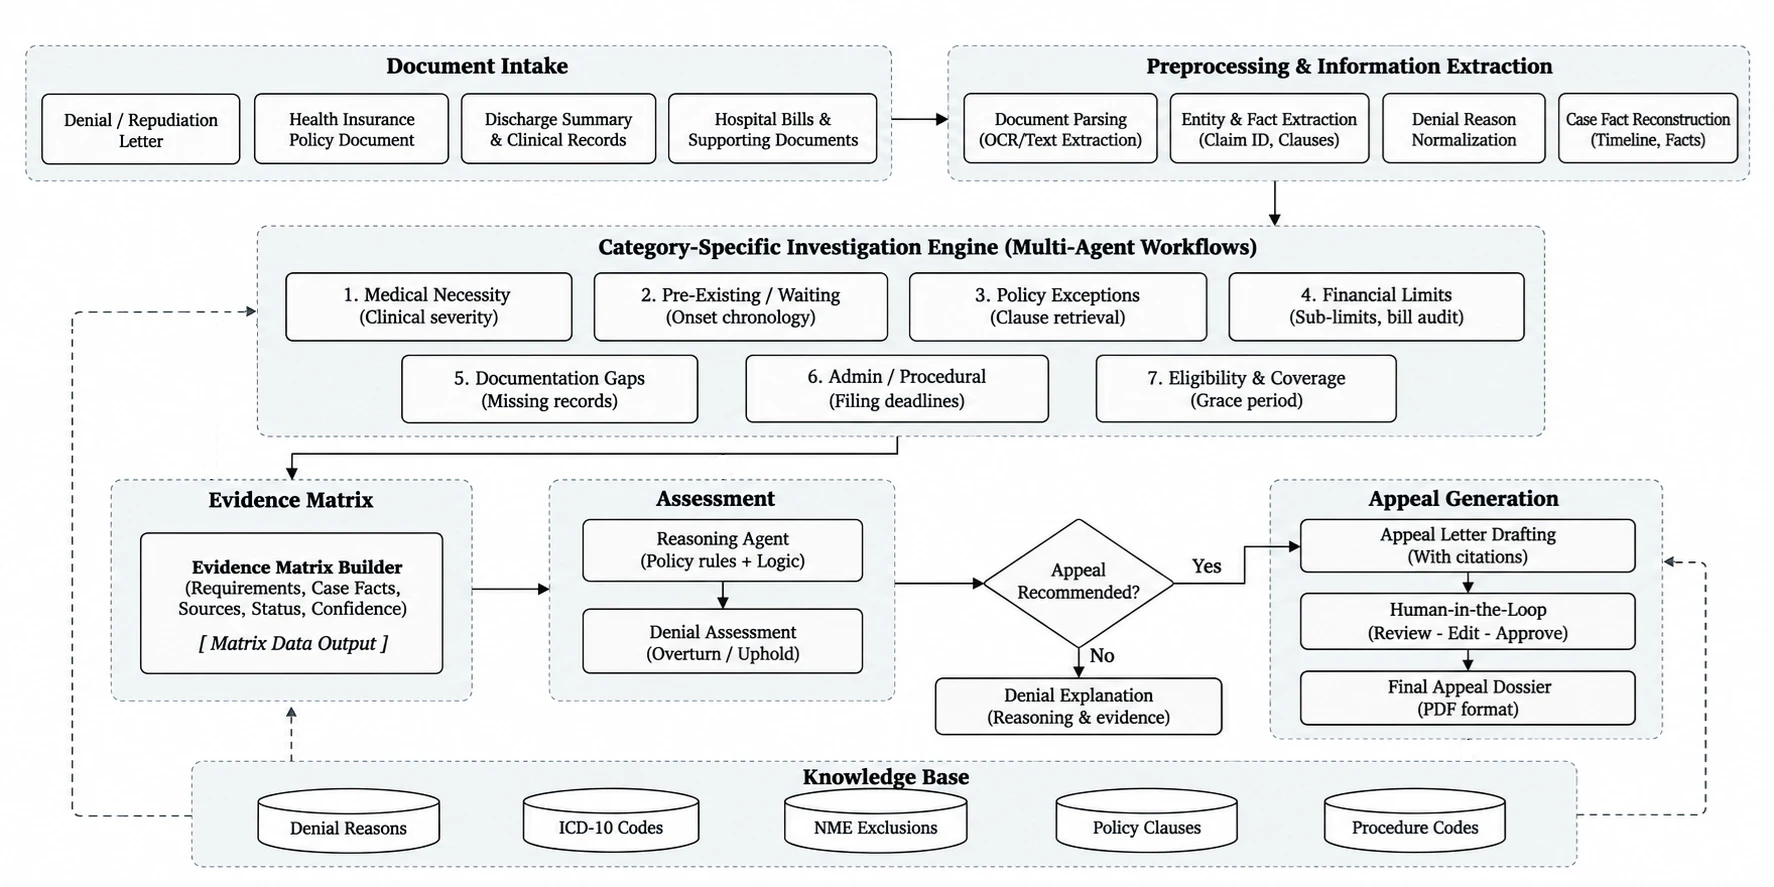
\includegraphics[width=\textwidth]{project_workflow.png}
\caption{Proposed system architecture for denial analysis and appeal support. The diagram shows the intended workflow and knowledge sources; its output is decision support for human review, not an automatic claim decision.}
\label{fig:system-architecture}
\end{figure*}

\subsection{Knowledge Resources}
The workflow uses six knowledge resources built from public sources. Table~\ref{tab:resources} lists each resource and the workflow stages that use it.

\begin{table}[!t]
\centering
\caption{Knowledge Resources Used by the Proposed Framework}
\label{tab:resources}
\scriptsize
\setlength{\tabcolsep}{3pt}
\renewcommand{\arraystretch}{1.15}
\begin{tabularx}{\columnwidth}{|P{1.7cm}|Y|P{2.3cm}|}
\hline
\textbf{Resource} & \textbf{Content} & \textbf{Used In} \\
\hline
Policy clause base & Clauses from 13 retail policy wordings of four Indian insurers, with type, exceptions, and time limits & Clause retrieval, exclusion and waiting-period checks, citation verification \\
\hline
Denial-reason taxonomy & Typical denial reasons in seven categories, with CARC/RARC codes, IRDAI provisions, and grievance routes & Denial categorization, forum selection \\
\hline
Diagnosis codes & Curated ICD-10-CM codes from all chapters, with billable status & Entity normalization, exclusion checks \\
\hline
Procedure codes & Curated CPT and HCPCS procedure codes with their code system & Entity normalization, sub-limit checks \\
\hline
Procedure--diagnosis map & Diagnoses that indicate each procedure, with the supporting CMS coverage policy & Medical-necessity investigation \\
\hline
Non-payable items schedule & Items in IRDAI Lists I to IV & Bill audit in financial-limit investigation \\
\hline
\end{tabularx}
\end{table}

The \emph{policy clause base} comes from the published wordings of 13 retail health insurance products sold by ICICI Lombard, Care Health, HDFC ERGO, and Star Health. Clauses are segmented using each document's own numbering and headings. Every record holds the insurer, product, section, clause number, clause text, and clause type (coverage, exclusion, definition, or waiting period), together with any time limit parsed into a structured value. Exception language such as ``except'', ``unless'', ``provided that'', or ``subject to'' is detected and the exception text is stored with its clause, so that an exclusion is never retrieved without its exception. The workflow searches this base when it looks up the clause cited in a denial, when it looks for exceptions, when it reads waiting periods and limits, and when it re-verifies citations before drafting.

The \emph{denial-reason taxonomy} lists typical denial reasons for each of the seven categories. Each reason carries its Claim Adjustment Reason Code (CARC) and Remittance Advice Remark Code (RARC) from the ASC X12 standard, the relevant IRDAI provision, and the Indian grievance route that applies: the insurer's grievance cell, the Insurance Ombudsman, or a consumer commission. The workflow uses it first to assign a denial to a category and again at the end to choose the forum for an appeal.

The \emph{diagnosis} and \emph{procedure code} tables are curated subsets of ICD-10-CM and of CPT and HCPCS, chosen for conditions and procedures that often appear in disputed claims. The diagnosis table records which codes are billable, and the procedure table records which coding system each code belongs to. Both are used during preprocessing to normalize the diagnoses and procedures found in clinical documents, and later to check them against exclusions and sub-limits. The \emph{procedure--diagnosis map} links each procedure to the diagnoses that indicate it and cites the U.S. Centers for Medicare \& Medicaid Services (CMS) coverage policy behind each link. The medical-necessity investigation uses it as a reference for clinical indications. Because these are U.S. policies, they do not bind Indian insurers. The \emph{non-payable items schedule} follows the four IRDAI lists: items for which no coverage is available (List~I) and items that are included in room, procedure, or treatment charges (Lists~II to IV). The financial-limit investigation uses it to audit bill deductions line by line.

\subsection{Evaluation Benchmarks}
If only the final appeal were evaluated, it would be hard to tell where an error came from. We therefore define a separate benchmark for each component, summarized in Table~\ref{tab:benchmarks}. The cases are synthetic. They are generated from templates whose values come from the policy wordings, the standard code sets, and public records of denials and appeals, and every ground-truth value can be traced to the case input or to a record in the knowledge resources.

\begin{table}[!t]
\centering
\caption{Component-Level Benchmarks}
\label{tab:benchmarks}
\scriptsize
\setlength{\tabcolsep}{3pt}
\renewcommand{\arraystretch}{1.15}
\begin{tabularx}{\columnwidth}{|P{1.45cm}|Y|P{1.55cm}|P{1.75cm}|}
\hline
\textbf{Benchmark} & \textbf{Ground Truth} & \textbf{Workflow Stage} & \textbf{Main Metrics} \\
\hline
Intake & Fields stated in each denial letter & Preprocessing & Field accuracy, exact match, token F1 \\
\hline
Clause retrieval & Governing clause and its exceptions in the clause base & Exclusion and waiting-period checks & Hit@$k$, MRR, context precision and recall \\
\hline
Clinical evidence & Checklist items and verbatim evidence spans & Medical-necessity investigation & Checklist accuracy, faithfulness \\
\hline
Chronology & Elapsed coverage, waiting-period and moratorium status & Waiting-period investigation & Exact match, date error \\
\hline
Reasoning & Toulmin components and verdict for all seven categories & Applicability and assessment & Verdict accuracy, completeness, judged soundness \\
\hline
Appeal drafting & Product-specific clause citations and evidence & Drafting & Citation precision and recall, edit ratio \\
\hline
Denial routing & Category of each denial paragraph & Denial categorization & Macro-F1, confusion matrix \\
\hline
\end{tabularx}
\end{table}

The \emph{intake} benchmark contains denial letters written in the format of Indian repudiation notices. Its ground truth lists the fields stated in each letter, including the claim identifier, patient, insurer and product, dates, amount, cited clause, and stated reason. It tests the preprocessing stage. The \emph{clause retrieval} benchmark pairs denial-style questions about a named product with the identifier of the governing clause in the clause base, the exceptions attached to it, and distractor clauses taken from the same product. It tests whether retrieval puts the controlling clause and its exceptions at the top, and is used whenever an investigation looks up policy text.

The \emph{clinical evidence} benchmark pairs clinical notes for common surgical and medical procedures with a medical-necessity checklist covering conservative treatment and its duration, disease severity, and physician certification. The evidence spans are copied verbatim from the notes, and each case has an expected determination, so that both extraction and judgment can be scored. The \emph{chronology} benchmark gives policy inception, symptom-onset, and admission dates, the declarations on the proposal form, the renewal history, and the applicable waiting period. Its ground truth is the elapsed coverage and the resulting waiting-period and moratorium status, computed under the moratorium rule of the current IRDAI health insurance regulations. It tests the date arithmetic in the waiting-period investigation.

The \emph{reasoning} benchmark gives, for each of the seven categories, the claim, grounds, warrant, exception status, and rebuttal of a Toulmin argument, together with the expected verdict. Cases where the denial is justified are included alongside cases where it should be reversed, so a system cannot score well by always favoring the policyholder. The \emph{appeal drafting} benchmark specifies, for each case, the product-specific clauses, evidence, and forum that a correct appeal must cite, along with a reference letter. The \emph{denial routing} benchmark contains denial paragraphs with distinct wording, balanced across the seven categories, each labeled with its category. It tests the categorization step.

\subsection{Evaluation Metrics}
Each metric measures one clearly defined property. For extraction and classification, \emph{precision} $P$ is the fraction of predicted items that are correct, \emph{recall} $R$ is the fraction of correct items that the system predicts, and the F1 score is their harmonic mean,
\begin{equation}
F_1 = \frac{2PR}{P+R}.
\label{eq:f1}
\end{equation}
For denial routing, the macro-averaged F1 score applies~\eqref{eq:f1} to each category $c$ and averages the results:
\begin{equation}
F_1^{\text{macro}} = \frac{1}{7}\sum_{c=1}^{7} F_{1,c}.
\label{eq:macrof1}
\end{equation}
Every category counts equally in~\eqref{eq:macrof1}. Real denials are unevenly spread across categories, and this keeps strong results on common categories from hiding failures on rare ones. The confusion matrix shows which categories the router mixes up, for example medical-necessity and exclusion denials.

For retrieval, Hit@$k$ is the fraction of queries for which a governing clause appears among the top $k$ results ($k \in \{1,3\}$). The mean reciprocal rank (MRR) rewards ranking that clause near the top:
\begin{equation}
\text{MRR} = \frac{1}{|Q|}\sum_{q \in Q}\frac{1}{\text{rank}_q},
\label{eq:mrr}
\end{equation}
where $Q$ is the set of queries and $\text{rank}_q$ is the position of the first governing clause for query $q$. Under~\eqref{eq:mrr} a clause ranked first contributes 1 and one ranked third contributes 1/3, so a perfect retriever scores 1. Context precision measures how much of the retrieved text is relevant, and context recall measures how much of the required information was retrieved~\cite{es2024}. The proposed retriever combines BM25 and dense rankings, so these metrics are reported for each retriever and for their combination by reciprocal rank fusion~\cite{cormack2009},
\begin{equation}
\text{RRF}(d) = \sum_{m \in M}\frac{1}{\kappa + \text{rank}_m(d)},
\label{eq:rrf}
\end{equation}
where $M$ is the set of retrievers, $\text{rank}_m(d)$ is the position of passage $d$ in the ranking produced by retriever $m$, and $\kappa$ is a smoothing constant, commonly 60. Equation~\eqref{eq:rrf} uses rank positions only, which lets it combine retrievers whose raw scores are on different scales.

Chronology decisions follow from date arithmetic, so the computed elapsed coverage must match the ground truth exactly, and any difference in days is reported as an error. For clinical evidence and appeal drafts, \emph{faithfulness} is the fraction of statements in the output that the source text supports~\cite{es2024}. \emph{Citation precision} is the share of citations that support their statements, and \emph{citation recall} is the share of required citations that appear~\cite{gao2023}. The edit ratio, based on the Levenshtein distance between the generated letter and the version the reviewer approves, estimates how much correction the reviewer had to make. Reasoning quality that cannot be checked exactly is scored with G-Eval~\cite{liu2023}, in which an LLM rates outputs against a written rubric.

The checks run at three levels. Level~1 uses deterministic comparisons such as exact match, date arithmetic, and F1. Level~2 uses an LLM as a judge against reference answers to score faithfulness and context recall. Level~3 evaluates the complete workflow, including citation support, with human review. LLM judges can be biased or inconsistent, so their scores are calibrated against a sample of human ratings and reported with agreement statistics.

\section{Limitations}
\label{sec:limitations}
The framework has not yet been implemented end to end, so no results are reported. The benchmarks are synthetic, and domain experts have yet to validate their ground truth. Real denial cases will be needed to show that results carry over to practice. The clause base holds one version of each of the 13 products, so changes between policy versions are not yet represented. The diagnosis codes follow ICD-10-CM and the clinical indications follow U.S. CMS policies, whereas Indian claims may use WHO ICD-10 and insurers may apply different clinical criteria. Most of the reviewed studies were also carried out in the United States, and their findings may not transfer directly to Indian denial practice and grievance procedures.

\section{Conclusion}
\label{sec:conclusion}
We reviewed research on policy knowledge extraction, retrieval of policy text, medical entity linkage, clinical evidence assessment, multi-agent medical-necessity assessment, denial triage, logic-based adjudication, and appeal generation. Each line of work has made progress on its own capability. Retrieval, outcome prediction, reasoning, and letter generation are separate tasks with different evaluation needs. Models often reach correct decisions without sound justifications, and generated letters often contain unsupported statements.

Appeal support that can be trusted has to keep a traceable link between the denial reason, the policy language that applies, the documented facts, the evidence still missing, and each statement in the appeal. The analysis must handle exceptions, record uncertainty, verify its citations, and leave the final judgment to a qualified person. A plausible letter or a relevant paragraph does not meet that standard. The proposed framework is built around these requirements. Its knowledge resources come from Indian policy wordings and public code sets, and its benchmarks test each component against ground truth that can be traced to the case documents or to the knowledge resources. Together they provide the means to test the framework empirically as its implementation proceeds.

\begin{thebibliography}{00}

\bibitem{lewis2020}
P.~Lewis \textit{et al.}, ``Retrieval-augmented generation for knowledge-intensive NLP tasks,'' in \emph{Proc. Adv. Neural Inf. Process. Syst. (NeurIPS)}, vol.~33, 2020, pp.~9459--9474.

\bibitem{kumar2010}
M.~Kumar, R.~Ghani, and Z.-S.~Mei, ``Data mining to predict and prevent errors in health insurance claims processing,'' in \emph{Proc. 16th ACM SIGKDD Int. Conf. Knowl. Discovery Data Mining}, 2010, pp.~65--74, doi: 10.1145/1835804.1835816.

\bibitem{lopez2021}
V.~L\'{o}pez \textit{et al.}, ``Towards protecting vital healthcare programs by extracting actionable knowledge from policy,'' in \emph{Findings Assoc. Comput. Linguistics: ACL-IJCNLP 2021}, 2021, pp.~3509--3521, doi: 10.18653/v1/2021.findings-acl.308.

\bibitem{picco2022}
G.~Picco \textit{et al.}, ``Learning insurance benefit rules from policy texts with small labeled data,'' in \emph{MEDINFO 2021: One World, One Health}, ser. Studies in Health Technology and Informatics, vol.~290, 2022, doi: 10.3233/SHTI220081.

\bibitem{sbodio2024}
M.~L.~Sbodio \textit{et al.}, ``Collaborative artificial intelligence system for investigation of healthcare claims compliance,'' \emph{Sci. Rep.}, vol.~14, Art. no.~11884, 2024, doi: 10.1038/s41598-024-62665-0.

\bibitem{robertson2009}
S.~Robertson and H.~Zaragoza, ``The probabilistic relevance framework: BM25 and beyond,'' \emph{Found. Trends Inf. Retr.}, vol.~4, no.~1--2, pp.~1--174, 2009, doi: 10.1561/1500000019.

\bibitem{cormack2009}
G.~V.~Cormack, C.~L.~A.~Clarke, and S.~Buettcher, ``Reciprocal rank fusion outperforms Condorcet and individual rank learning methods,'' in \emph{Proc. 32nd Int. ACM SIGIR Conf. Res. Develop. Inf. Retr.}, 2009, pp.~758--759, doi: 10.1145/1571941.1572114.

\bibitem{hanmante2026}
S.~Hanmante, S.~Patil, P.~V.~Deshmukh, and A.~K.~Shahade, ``InsuranceRAG: A multi-module retrieval-augmented AI system for intelligent insurance assistance,'' \emph{Softw. Impacts}, vol.~28, Art. no.~100844, 2026, doi: 10.1016/j.simpa.2026.100844.

\bibitem{zhang2020}
T.~Zhang, V.~Kishore, F.~Wu, K.~Q.~Weinberger, and Y.~Artzi, ``BERTScore: Evaluating text generation with BERT,'' in \emph{Proc. Int. Conf. Learn. Represent. (ICLR)}, 2020.

\bibitem{kamel2024}
S.~J.~Lui, C.~Xiang, and S.~Krishnaswamy, ``KAMEL: Knowledge aware medical entity linkage to automate health insurance claims processing,'' in \emph{Proc. AAAI Conf. Artif. Intell.}, vol.~38, no.~21, 2024, pp.~22797--22805, doi: 10.1609/aaai.v38i21.30314.

\bibitem{lui2024}
S.~J.~Lui, C.~Xiang, and S.~Krishnaswamy, ``Knowledge aware automated health claims processing with medical ontologies and large language models,'' in \emph{Proc. AAAI Symp. Ser.}, vol.~4, no.~1, 2024, pp.~199--209, doi: 10.1609/aaaiss.v4i1.31794.

\bibitem{ahsan2023}
H.~Ahsan \textit{et al.}, ``Retrieving evidence from EHRs with LLMs: Possibilities and challenges,'' in \emph{Proc. Conf. Health, Inference, Learn. (CHIL)}, ser. Proc. Mach. Learn. Res., vol.~248, 2024, pp.~489--505.

\bibitem{pandey2024}
H.~G.~Pandey, A.~Amod, and S.~Kumar, ``Advancing healthcare automation: Multi-agent system for medical necessity justification,'' in \emph{Proc. 23rd Workshop Biomed. Natural Lang. Process. (BioNLP)}, Bangkok, Thailand, 2024, pp.~39--49, doi: 10.18653/v1/2024.bionlp-1.4.

\bibitem{owolabi2025}
T.~Owolabi, ``Transforming appeal decisions: Machine learning triage for hospital admission denials,'' \emph{JAMIA Open}, vol.~8, no.~1, Art. no.~ooaf016, 2025, doi: 10.1093/jamiaopen/ooaf016.

\bibitem{prakken2015}
H.~Prakken and G.~Sartor, ``Law and logic: A review from an argumentation perspective,'' \emph{Artif. Intell.}, vol.~227, pp.~214--245, Oct. 2015, doi: 10.1016/j.artint.2015.06.005.

\bibitem{toulmin2003}
S.~E.~Toulmin, \emph{The Uses of Argument}, updated ed. Cambridge, U.K.: Cambridge Univ. Press, 2003, doi: 10.1017/CBO9780511840005.

\bibitem{inslogicbench2026}
J.~Liu \textit{et al.}, ``InsLogicBench: An argumentation logic grounded benchmark for complex insurance claims adjudication,'' in \emph{Proc. 64th Annu. Meeting Assoc. Comput. Linguistics (Vol. 1: Long Papers)}, 2026, pp.~22592--22619, doi: 10.18653/v1/2026.acl-long.1035.

\bibitem{pokharel2026}
R.~Pokharel, H.~R.~Hassanzadeh, and A.~Agrawal, ``From policy to logic for efficient and interpretable coverage assessment,'' presented at the AAAI Workshop AI for Medicine and Healthcare (AIMedHealth), 2026, arXiv:2601.01266.

\bibitem{kiser2024}
K.~J.~Kiser, M.~Waters, J.~Reckford, C.~Lundeberg, and C.~D.~Abraham, ``Large language models to help appeal denied radiotherapy services,'' \emph{JCO Clin. Cancer Inform.}, vol.~8, Art. no.~e2400129, 2024, doi: 10.1200/CCI.24.00129.

\bibitem{deniedai2026}
C.~J.~McCarthy \textit{et al.}, ``Decreasing administrative effort related to non-approval of image-guided procedures using large language models---The DENIED-AI pilot study,'' \emph{Acad. Radiol.}, vol.~33, no.~8, pp.~3221--3231, 2026, doi: 10.1016/j.acra.2026.04.021.

\bibitem{ji2023}
Z.~Ji \textit{et al.}, ``Survey of hallucination in natural language generation,'' \emph{ACM Comput. Surv.}, vol.~55, no.~12, pp.~1--38, 2023, doi: 10.1145/3571730.

\bibitem{gao2023}
T.~Gao, H.~Yen, J.~Yu, and D.~Chen, ``Enabling large language models to generate text with citations,'' in \emph{Proc. Conf. Empirical Methods Natural Lang. Process. (EMNLP)}, 2023, pp.~6465--6488, doi: 10.18653/v1/2023.emnlp-main.398.

\bibitem{es2024}
S.~Es, J.~James, L.~Espinosa Anke, and S.~Schockaert, ``RAGAs: Automated evaluation of retrieval augmented generation,'' in \emph{Proc. 18th Conf. Eur. Chapter Assoc. Comput. Linguistics: Syst. Demonstrations}, 2024, pp.~150--158, doi: 10.18653/v1/2024.eacl-demo.16.

\bibitem{parasuraman2010}
R.~Parasuraman and D.~H.~Manzey, ``Complacency and bias in human use of automation: An attentional integration,'' \emph{Hum. Factors}, vol.~52, no.~3, pp.~381--410, 2010, doi: 10.1177/0018720810376055.

\bibitem{liu2023}
Y.~Liu, D.~Iter, Y.~Xu, S.~Wang, R.~Xu, and C.~Zhu, ``G-Eval: NLG evaluation using GPT-4 with better human alignment,'' in \emph{Proc. Conf. Empirical Methods Natural Lang. Process. (EMNLP)}, 2023, pp.~2511--2522, doi: 10.18653/v1/2023.emnlp-main.153.

\end{thebibliography}

\end{document}
